%%%%%%%%%%%%%%%%%%%%%%%%%%%%%%%%%%%%%%%%%%%%%%%%%%%%%%%%%%%%%%%%%%%%%%%%%%
\chapter{Závěr}


V~této práci jsem se zabývala hlubokými zásobníkovými automaty z~pohledu počtu nevstupních symbolů a stavů. Cílem bylo zavést nové modifikace tohoto typu automatu a dosáhnout tak jeho částečného zjednodušení. Po dohodě s~vedoucím práce jsem původní zadání rozšířila o~problematiku normální formy a zobecněné varianty hlubokých zásobníkových automatů.

Dokázala jsem, že hluboký zásobníkový automat konečného indexu s~jedním nevstupním symbolem je ekvivalentní s~programovými gramatikami konečného indexu. Znamená to, že omezením počtu nevstupních symbolů na jeden se jeho mocnost nezměnila.  Dále jsem zavedla normální formu hlubokého zásobníkového automatu se čtyřmi typy pravidel a docílila tak zjednodušení jejich zápisu. Nakonec jsem definovala zobecněný hluboký zásobníkový automat. Toto zobecnění spočívá v~odstranění hloubky expanze z~pravidel. Místo toho je upraveno chování automatu tak, aby expandoval nejvrchnější možný nevstupní symbol na svém zásobníku. Tento typ automatu s~povolenými $\varepsilon$-pravidly má mocnost Turingova stroje a platí, že zredukováním počtu nevstupních symbolů, případně stavů, na tři se síla automatu nezmění. Srovnání mocností zavedených automatů a zasazení do širšího kontextu je k~dispozici na diagramu \ref{obr_model02_hierarchy}.


Algoritmy pro redukci zobecněného hlubokého zásobníkového automatu jsem po dohodě s~vedoucím práce implementovala v~konzolové aplikaci \texttt{gdeep\_pda}. Ta umožňuje převádět vstupní automat na zredukovaný, případně provést syntaktickou analýzu vstupního řetězce, a výsledek vypsat na výstup. Aplikace je implementovaná v~jazyce Python a slouží k~demonstračním účelům. 

Uvedené algoritmy popisují, jakým způsobem je možné jeden model převést na druhý, z~čehož lze vyvozovat závěry o~jejich ekvivalenci. Bylo by však vhodné ověřit správnost algoritmů formálním způsobem. Z~navržených redukcí lze dále odvodit, že omezení počtu prvků jedné komponenty automatu se projevuje výrazným zvýšením počtu prvků v~ostatních komponentách. Konkrétně, když jsem omezila počet nevstupních symbolů, zvýšila se kardinalita množin pravidel a stavů a po omezení počtu stavů, narostla kardinalita množin pravidel a nevstupních symbolů. Je tedy pravděpodobné, že není možné současně omezit počet stavů a počet nevstupních symbolů se zachováním mocnosti automatu. Jedná se však o~zajímavou problematiku vhodnou k~dalšímu prostudování.



\begin{figure}[ht]
\centering
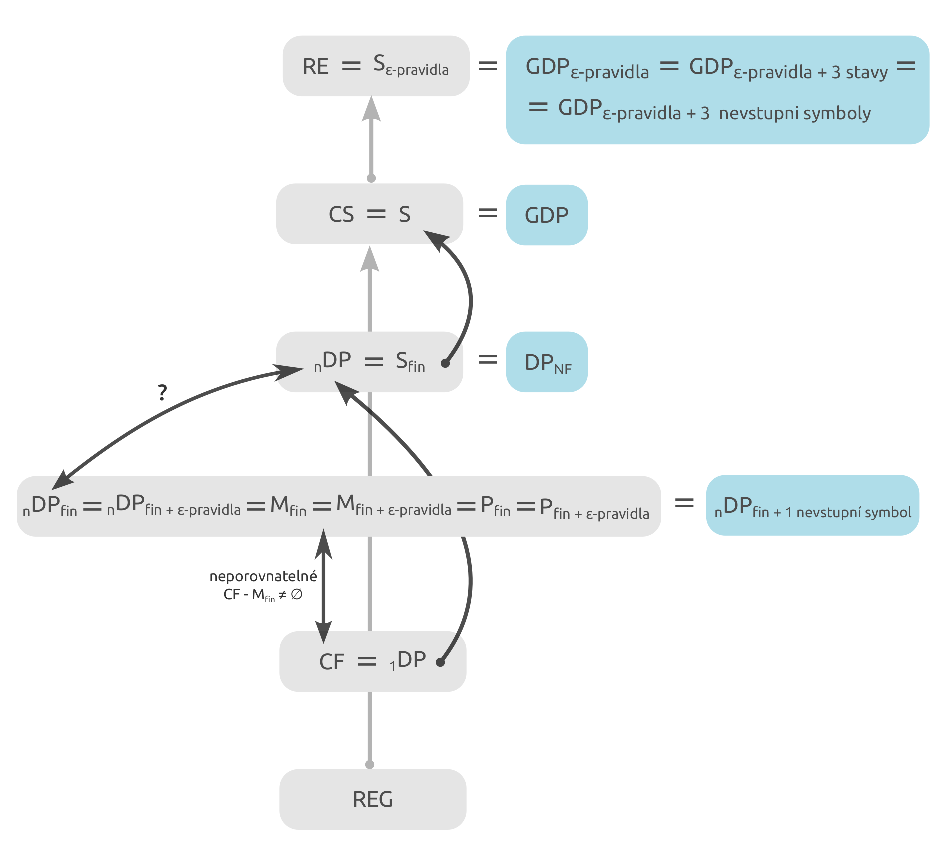
\includegraphics{img/bp_hierarchy03.eps} \bigskip \\
\caption{Zařazení automatů do kontextu jazykových rodin. Význam jednotlivých zkratek je vysvětlen v~kapitole \ref{kap_teorie_hierarchie}. Dále \textbf{DP${}_{NF}$} označuje rodinu jazyků přijímaných hlubokými zásobníkovými automaty v~normální formě a \textbf{GDP} rodinu jazyků přijímaných zobecněnými hlubokými zásobníkovými automaty.}
\label{obr_model02_hierarchy}
\end{figure}

%=========================================================================

